\documentclass[12pt, smalloffset, compress, aspectratio=1610]{beamer}

\usetheme{pl}

\usepackage[copies]{contour}

\usepackage{longtable}
\usepackage{booktabs}
\usepackage{tabularx}
\usepackage{minted}
\usepackage{listings}
\usepackage{color}
\usepackage{fancyvrb}
\newcommand{\VerbBar}{|}
\newcommand{\VERB}{\Verb[commandchars=\\\{\}]}
\DefineVerbatimEnvironment{Highlighting}{Verbatim}{commandchars=\\\{\},fontsize=\small}
% Add ',fontsize=\small' for more characters per line
\usepackage[framemethod=tikz]{mdframed}
\definecolor{shadecolor}{HTML}{EEEEEE}
\mdfsetup{
  backgroundcolor=shadecolor,
  linecolor=shadecolor,
  innerleftmargin=5pt,
  innerrightmargin=5pt,
  leftmargin=-5pt,
  rightmargin=-5pt,
  roundcorner=3pt
}
\newenvironment{Shaded}{\begin{mdframed}}{\end{mdframed}}
\newcommand{\KeywordTok}[1]{\textcolor[rgb]{0.26,0.66,0.93}{\textbf{{#1}}}}
\newcommand{\DataTypeTok}[1]{\textcolor[rgb]{0.74,0.68,0.62}{\underline{{#1}}}}
\newcommand{\DecValTok}[1]{\textcolor[HTML]{558B2F}{{#1}}}
\newcommand{\BaseNTok}[1]{\textcolor[HTML]{558B2F}{{#1}}}
\newcommand{\FloatTok}[1]{\textcolor[HTML]{558B2F}{{#1}}}
\newcommand{\ConstantTok}[1]{\textcolor[rgb]{0.74,0.68,0.62}{{#1}}}
\newcommand{\CharTok}[1]{\textcolor[HTML]{7E57C2}{{#1}}}
\newcommand{\SpecialCharTok}[1]{\textcolor[HTML]{7E57C2}{{#1}}}
\newcommand{\StringTok}[1]{\textcolor[HTML]{7E57C2}{{#1}}}
\newcommand{\VerbatimStringTok}[1]{\textcolor[HTML]{7E57C2}{{#1}}}
\newcommand{\SpecialStringTok}[1]{\textcolor[HTML]{7E57C2}{{#1}}}
\newcommand{\ImportTok}[1]{\textcolor[rgb]{0.74,0.68,0.62}{{#1}}}
\newcommand{\CommentTok}[1]{\textcolor[HTML]{546E7A}{\textit{{#1}}}}
\newcommand{\DocumentationTok}[1]{\textcolor[HTML]{BCAAA4}{\textit{{#1}}}}
\newcommand{\AnnotationTok}[1]{\textcolor[HTML]{BCAAA4}{\textbf{\textit{{#1}}}}}
\newcommand{\CommentVarTok}[1]{\textcolor[rgb]{0.74,0.68,0.62}{{#1}}}
\newcommand{\OtherTok}[1]{\textcolor[rgb]{0.74,0.68,0.62}{{#1}}}
\newcommand{\FunctionTok}[1]{\textcolor[HTML]{26A69A}{\textbf{{#1}}}}
\newcommand{\VariableTok}[1]{\textcolor[rgb]{0.74,0.68,0.62}{{#1}}}
\newcommand{\ControlFlowTok}[1]{\textcolor[rgb]{0.26,0.66,0.93}{\textbf{{#1}}}}
\newcommand{\OperatorTok}[1]{\textcolor[rgb]{0.74,0.68,0.62}{{#1}}}
\newcommand{\BuiltInTok}[1]{\textcolor[HTML]{42A5F5}{{#1}}}
\newcommand{\ExtensionTok}[1]{\textcolor[rgb]{0.74,0.68,0.62}{{#1}}}
\newcommand{\PreprocessorTok}[1]{\textcolor[rgb]{0.74,0.68,0.62}{\textbf{{#1}}}}
\newcommand{\AttributeTok}[1]{\textcolor[rgb]{0.74,0.68,0.62}{{#1}}}
\newcommand{\RegionMarkerTok}[1]{\textcolor[rgb]{0.74,0.68,0.62}{{#1}}}
\newcommand{\InformationTok}[1]{\textcolor[rgb]{0.00,0.40,1.00}{\textbf{\textit{{#1}}}}}
\newcommand{\WarningTok}[1]{\textcolor[HTML]{FF6E40}{\textbf{{#1}}}}
\newcommand{\AlertTok}[1]{\textcolor[HTML]{FF3D00}{{#1}}}
\newcommand{\ErrorTok}[1]{\textcolor[HTML]{DD2C00}{\textbf{{#1}}}}
\newcommand{\NormalTok}[1]{\textcolor[HTML]{212121}{{#1}}}

\makeatletter
\newsavebox\pandoc@box
\newcommand*\pandocbounded[1]{% scales image to fit in text height/width
  \sbox\pandoc@box{#1}%
  \Gscale@div\@tempa{0.8\textheight}{\dimexpr\ht\pandoc@box+\dp\pandoc@box\relax}%
  \Gscale@div\@tempb{\linewidth}{\wd\pandoc@box}%
  \ifdim\@tempb\p@<\@tempa\p@\let\@tempa\@tempb\fi% select the smaller of both
  \ifdim\@tempa\p@<\p@\scalebox{\@tempa}{\usebox\pandoc@box}%
  \else\usebox{\pandoc@box}%
  \fi%
}
% Set default figure placement to htbp
\def\fps@figure{htbp}
\makeatother

\providecommand{\tightlist}{%
  \setlength{\itemsep}{0pt}\setlength{\parskip}{0pt}}

\let\OldTexttt\texttt
\renewcommand{\texttt}[1]{\OldTexttt{\color{codecolor}#1}}

\makeatletter
\def\maxwidth{\ifdim\Gin@nat@width>\linewidth\linewidth\else\Gin@nat@width\fi}
\makeatother

\newcommand{\begincols}{\begin{columns}}
\newcommand{\stopcols}{\end{columns}}
\newcommand{\roundpicture}[2]{%
\tikz\node[circle,
          text=white,
          minimum width=4cm,
          minimum height=4cm,
          path picture={
              \node at (path picture bounding box.center){
                  \includegraphics[width=4cm]{#1}
              };
          }]{#2};
}
\newcommand{\plain}[1]{%
\begin{tikzpicture}[remember picture, overlay]
    \node at (current page.north west) [anchor = north west, inner sep = 0pt, outer sep = 0pt] {%
        \pgfuseimage{titlebackground};%
    };

\node at (current page.north west) [anchor = north west, inner sep = 0pt, outer sep = 0pt] {%
                \tikz {\draw [very nearly opaque, backgroundcolor, fill=backgroundcolor] (0,0) rectangle (12,10);}%
            };
            \node at (current page.west) [anchor = west, inner sep = 0cm, outer sep = 0cm, align=left, xshift=1.5cm] {%
                \Large
                #1
            };
        \end{tikzpicture}
}

\title{Interpretable ML for biodiversity}
\subtitle{An introduction using species distribution models}
\date{\today}
\author{Timothée Poisot}
\institute{Université de Montréal}

\begin{document}

\begin{frame}{Main goals}
\phantomsection\label{main-goals}
\begin{enumerate}
\tightlist
\item
  How do we produce a model?
\item
  How do we convey that it works?
\item
  How do we talk about how it makes predictions?
\item
  How do we use it to guide actions?
\end{enumerate}
\end{frame}

\begin{frame}{The steps}
\phantomsection\label{the-steps}
\begin{enumerate}
\tightlist
\item
  Get data about species occurrences
\item
  Build a classifier and make it as good as we can
\item
  Measure its performance
\item
  Explain some predictions
\item
  Generate counterfactual explanations
\item
  Briefly discuss ensemble models
\end{enumerate}
\end{frame}

\begin{frame}{But why\ldots{}}
\phantomsection\label{but-why}
\begin{description}
\tightlist
\item[\ldots{} think of SDM as a ML problem?]
Because they are! We want to learn a predictive algorithm from data
\item[\ldots{} the focus on explainability?]
We cannot ask people to \emph{trust} - we must \emph{convince} and
\emph{explain}
\end{description}
\end{frame}

\section{Problem statement}\label{problem-statement}

\begin{frame}{The problem in ecological terms}
\phantomsection\label{the-problem-in-ecological-terms}
We have information about a species
\end{frame}

\begin{frame}{The problem in other words}
\phantomsection\label{the-problem-in-other-words}
We have a series of observations \(y \in \mathbb{B}\), and predictors
variables \(\mathbf{X} \in \mathbb{R}\)

We want to find an algorithm \(f(\mathbf{x}) = \hat y\) that results in
the distance between \(\hat y\) and \(y\) being \emph{small}
\end{frame}

\begin{frame}{Setting up the data for our example}
\phantomsection\label{setting-up-the-data-for-our-example}
The predictor data will come from CHELSA2 - we will start with the 19
BioClim variables

We will use data on observations of \emph{Turdus torquatus} in
Switzerland, downloaded from the copy of the eBird dataset on GBIF
\end{frame}

\begin{frame}{The observation data}
\phantomsection\label{the-observation-data}
\pandocbounded{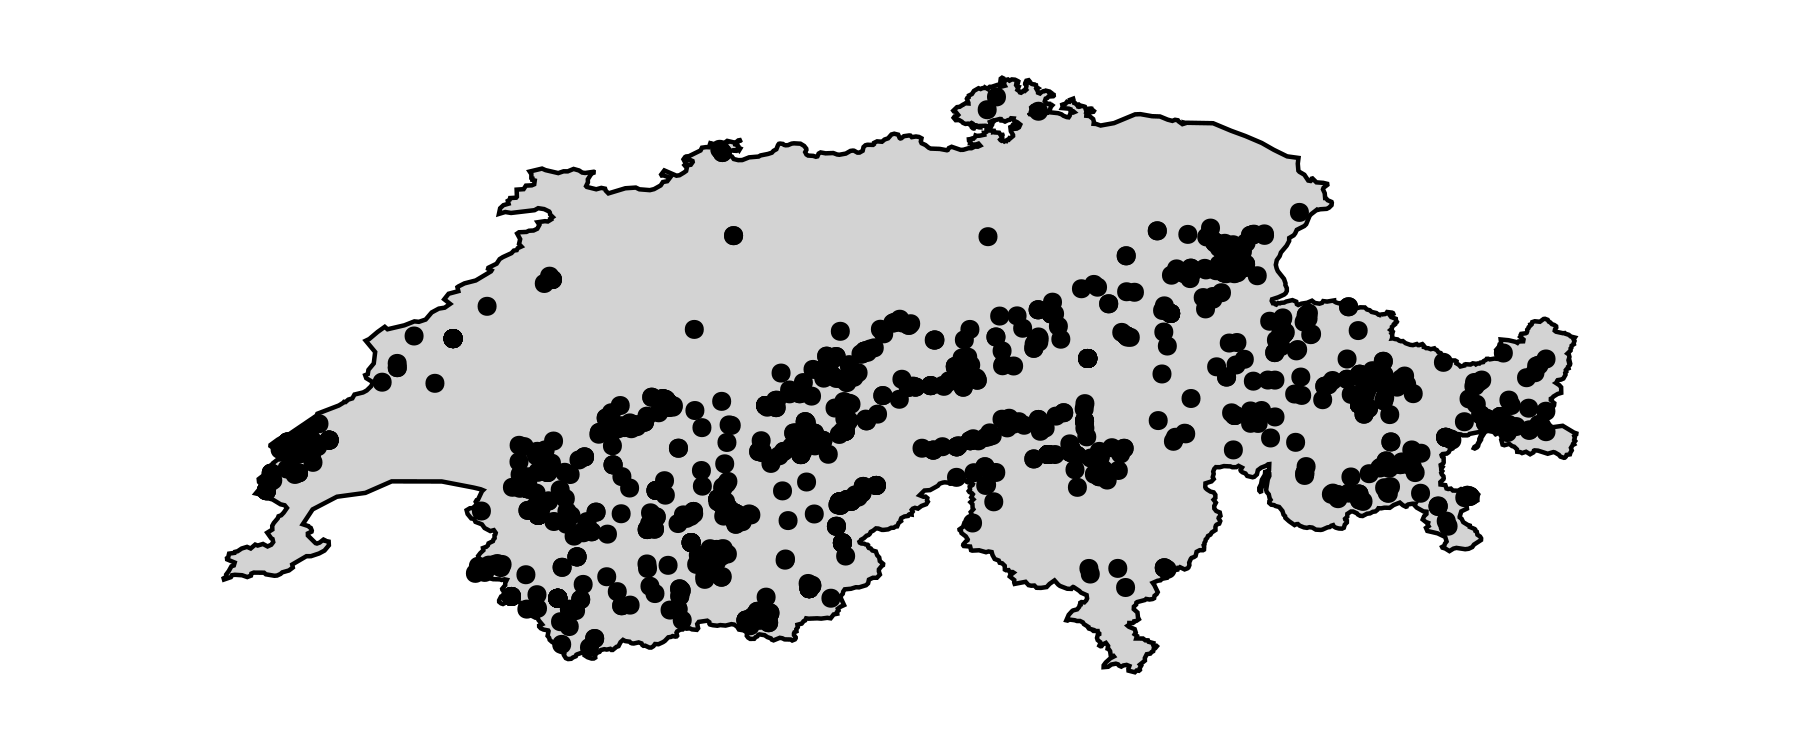
\includegraphics[keepaspectratio]{figures/slides_4_1.png}}~
\end{frame}

\begin{frame}{Problem!}
\phantomsection\label{problem}
We want \(\hat y \in \mathbb{B}\), and so far we are missing
\alert{negative values}
\end{frame}

\begin{frame}{Solution!}
\phantomsection\label{solution}
pseudo-absences

what are the assumptions we make
\end{frame}

\begin{frame}{The (inflated) observation data}
\phantomsection\label{the-inflated-observation-data}
\pandocbounded{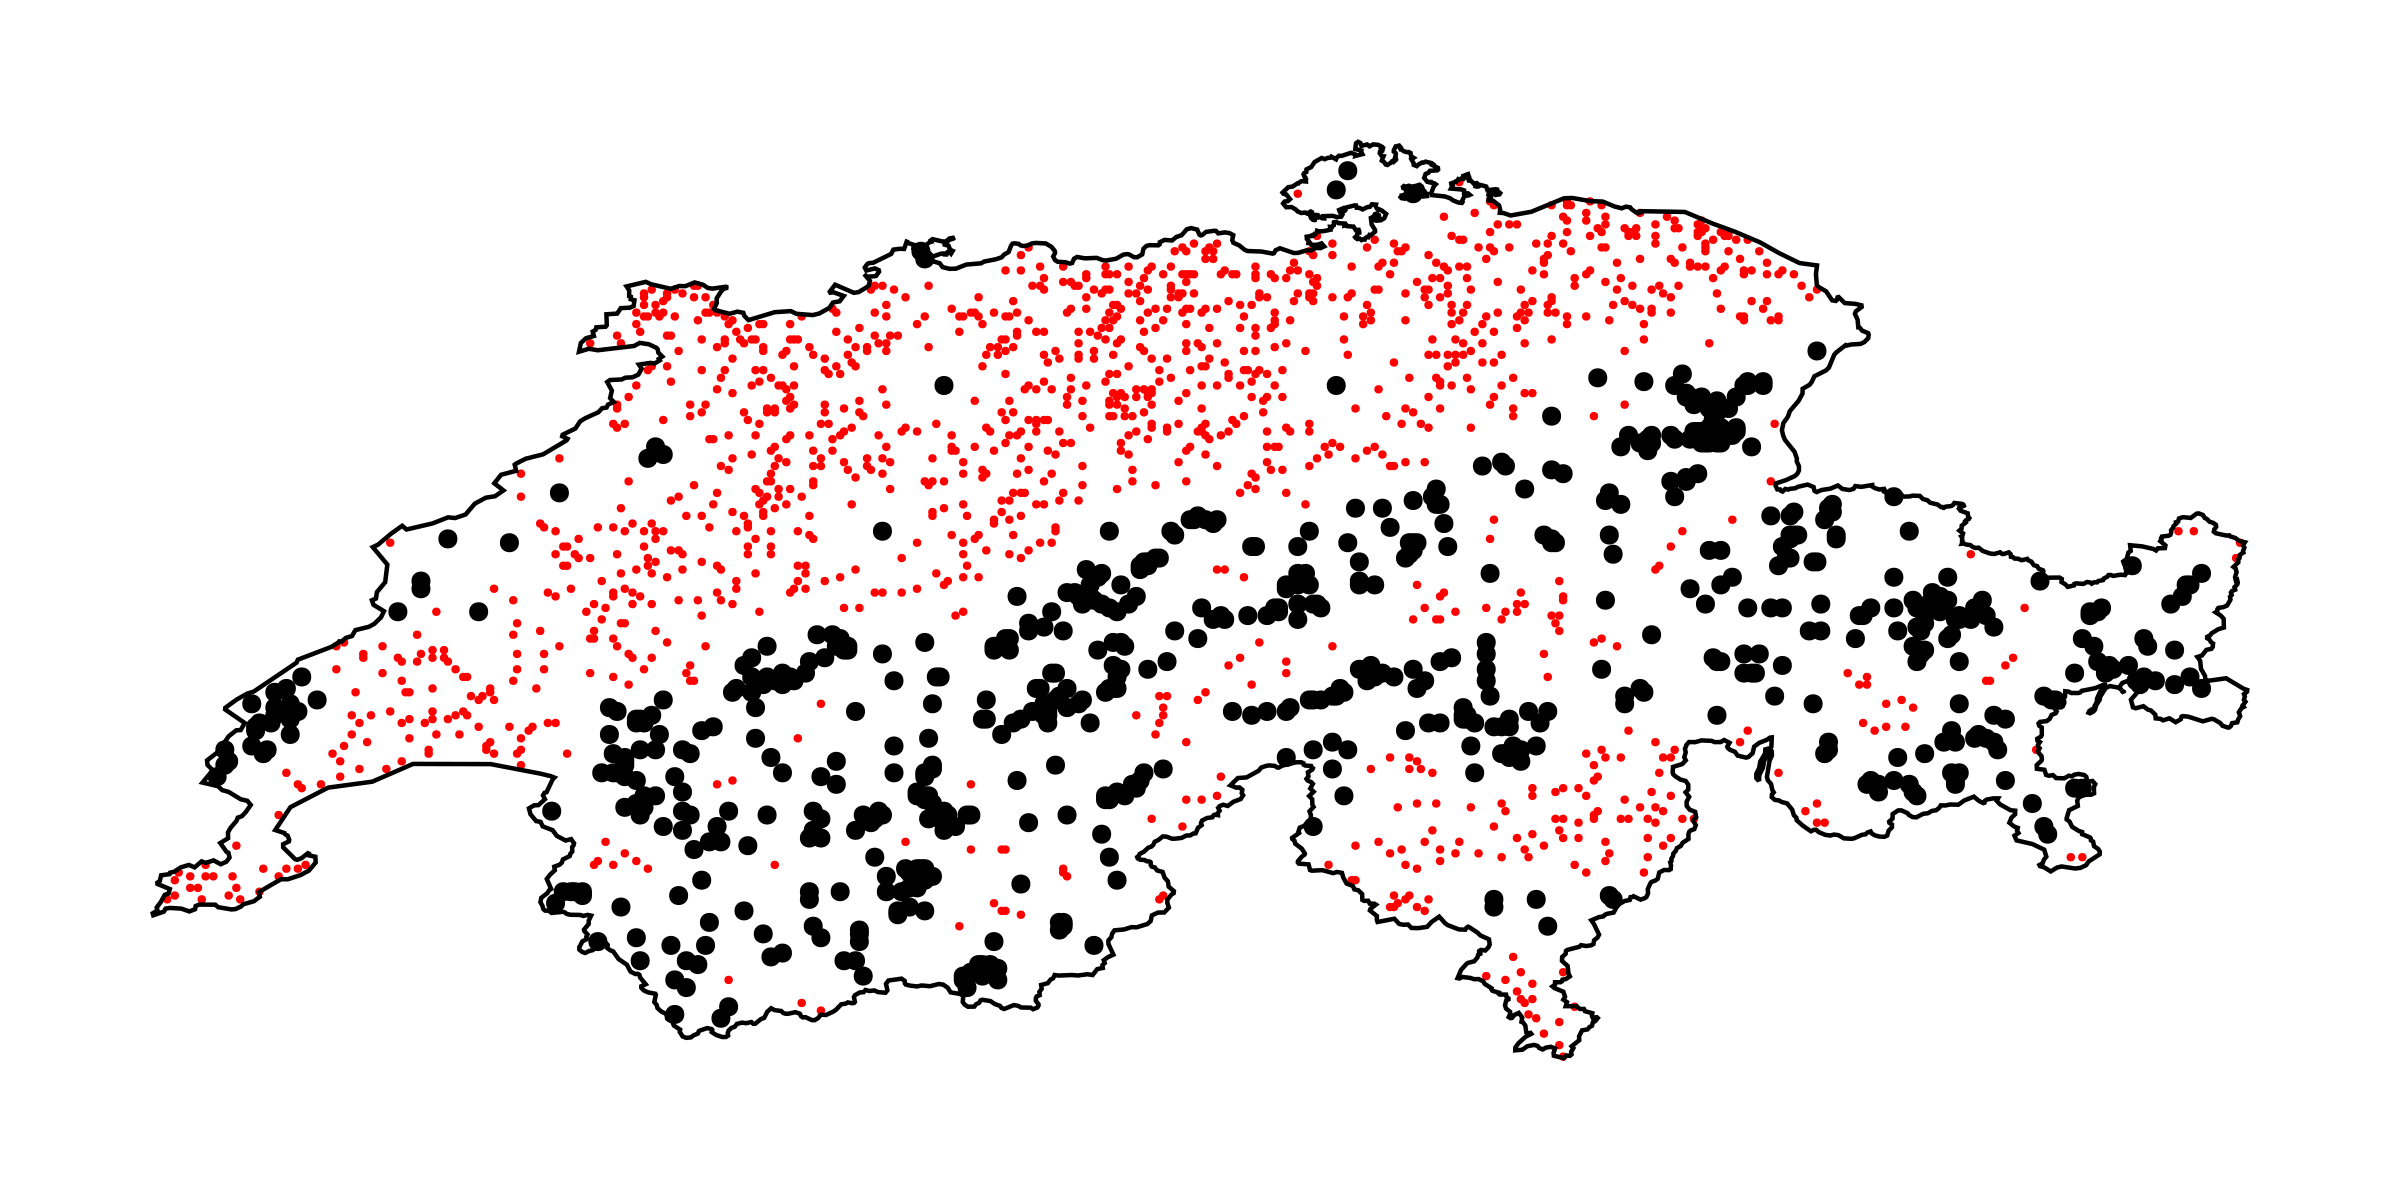
\includegraphics[keepaspectratio]{figures/slides_6_1.png}}~
\end{frame}

\section{Training the model}\label{training-the-model}

\begin{frame}{The Naive Bayes Classifier}
\phantomsection\label{the-naive-bayes-classifier}
\[P(+|x) = \frac{P(+)}{P(x)}P(x|+)\]

\[\hat y = \text{argmax}_j \, P(\mathbf{c}_j)\prod_i P(\mathbf{x}_i|\mathbf{c}_j)\]

\[P(x|+) = \text{pdf}(x, \mathcal{N}(\mu_+, \sigma_+))\]
\end{frame}

\begin{frame}{Setup}
\phantomsection\label{setup}
\end{frame}

\begin{frame}{Cross-validation}
\phantomsection\label{cross-validation}
Can we train the model

assumes parallel universes with slightly less data

is the model good?
\end{frame}

\begin{frame}{Null classifiers}
\phantomsection\label{null-classifiers}
coin flip

no skill

constant
\end{frame}

\begin{frame}{Expectations}
\phantomsection\label{expectations}
\begin{longtable}[]{@{}
  >{\raggedleft\arraybackslash}p{(\linewidth - 10\tabcolsep) * \real{0.2466}}
  >{\raggedleft\arraybackslash}p{(\linewidth - 10\tabcolsep) * \real{0.1507}}
  >{\raggedleft\arraybackslash}p{(\linewidth - 10\tabcolsep) * \real{0.1370}}
  >{\raggedleft\arraybackslash}p{(\linewidth - 10\tabcolsep) * \real{0.1370}}
  >{\raggedleft\arraybackslash}p{(\linewidth - 10\tabcolsep) * \real{0.1370}}
  >{\raggedleft\arraybackslash}p{(\linewidth - 10\tabcolsep) * \real{0.1918}}@{}}
\toprule\noalign{}
\begin{minipage}[b]{\linewidth}\raggedleft
\textbf{Model}
\end{minipage} & \begin{minipage}[b]{\linewidth}\raggedleft
\textbf{MCC}
\end{minipage} & \begin{minipage}[b]{\linewidth}\raggedleft
\textbf{PPV}
\end{minipage} & \begin{minipage}[b]{\linewidth}\raggedleft
\textbf{NPV}
\end{minipage} & \begin{minipage}[b]{\linewidth}\raggedleft
\textbf{DOR}
\end{minipage} & \begin{minipage}[b]{\linewidth}\raggedleft
\textbf{Accuracy}
\end{minipage} \\
\midrule\noalign{}
\endhead
noskill & 0.0 & 0.338178 & 0.661822 & 1.0 & 0.552373 \\
coinflip & -0.323643 & 0.338178 & 0.338178 & 0.261102 & 0.338178 \\
constantpositive & 0.0 & 0.338178 & NaN & NaN & 0.338178 \\
constantnegative & 0.0 & NaN & 0.661822 & NaN & 0.661822 \\
\bottomrule\noalign{}
\end{longtable}
\end{frame}

\begin{frame}{Cross-validation strategy}
\phantomsection\label{cross-validation-strategy}
k-fold

validation / training / testing
\end{frame}

\begin{frame}{Cross-validation results}
\phantomsection\label{cross-validation-results}
\begin{longtable}[]{@{}
  >{\raggedleft\arraybackslash}p{(\linewidth - 10\tabcolsep) * \real{0.2466}}
  >{\raggedleft\arraybackslash}p{(\linewidth - 10\tabcolsep) * \real{0.1507}}
  >{\raggedleft\arraybackslash}p{(\linewidth - 10\tabcolsep) * \real{0.1370}}
  >{\raggedleft\arraybackslash}p{(\linewidth - 10\tabcolsep) * \real{0.1370}}
  >{\raggedleft\arraybackslash}p{(\linewidth - 10\tabcolsep) * \real{0.1370}}
  >{\raggedleft\arraybackslash}p{(\linewidth - 10\tabcolsep) * \real{0.1918}}@{}}
\toprule\noalign{}
\begin{minipage}[b]{\linewidth}\raggedleft
\textbf{Model}
\end{minipage} & \begin{minipage}[b]{\linewidth}\raggedleft
\textbf{MCC}
\end{minipage} & \begin{minipage}[b]{\linewidth}\raggedleft
\textbf{PPV}
\end{minipage} & \begin{minipage}[b]{\linewidth}\raggedleft
\textbf{NPV}
\end{minipage} & \begin{minipage}[b]{\linewidth}\raggedleft
\textbf{DOR}
\end{minipage} & \begin{minipage}[b]{\linewidth}\raggedleft
\textbf{Accuracy}
\end{minipage} \\
\midrule\noalign{}
\endhead
noskill & 0.0 & 0.338178 & 0.661822 & 1.0 & 0.552373 \\
coinflip & -0.323643 & 0.338178 & 0.338178 & 0.261102 & 0.338178 \\
constantpositive & 0.0 & 0.338178 & NaN & NaN & 0.338178 \\
constantnegative & 0.0 & NaN & 0.661822 & NaN & 0.661822 \\
Validation & 0.285042 & 0.573912 & 0.739042 & 3.97394 & 0.698661 \\
Training & 0.287722 & 0.57633 & 0.73963 & 3.869 & 0.699451 \\
\bottomrule\noalign{}
\end{longtable}
\end{frame}

\begin{frame}{What to do if the model is trainable?}
\phantomsection\label{what-to-do-if-the-model-is-trainable}
train it!

re-use the full dataset
\end{frame}

\begin{frame}{Initial prediction}
\phantomsection\label{initial-prediction}
\pandocbounded{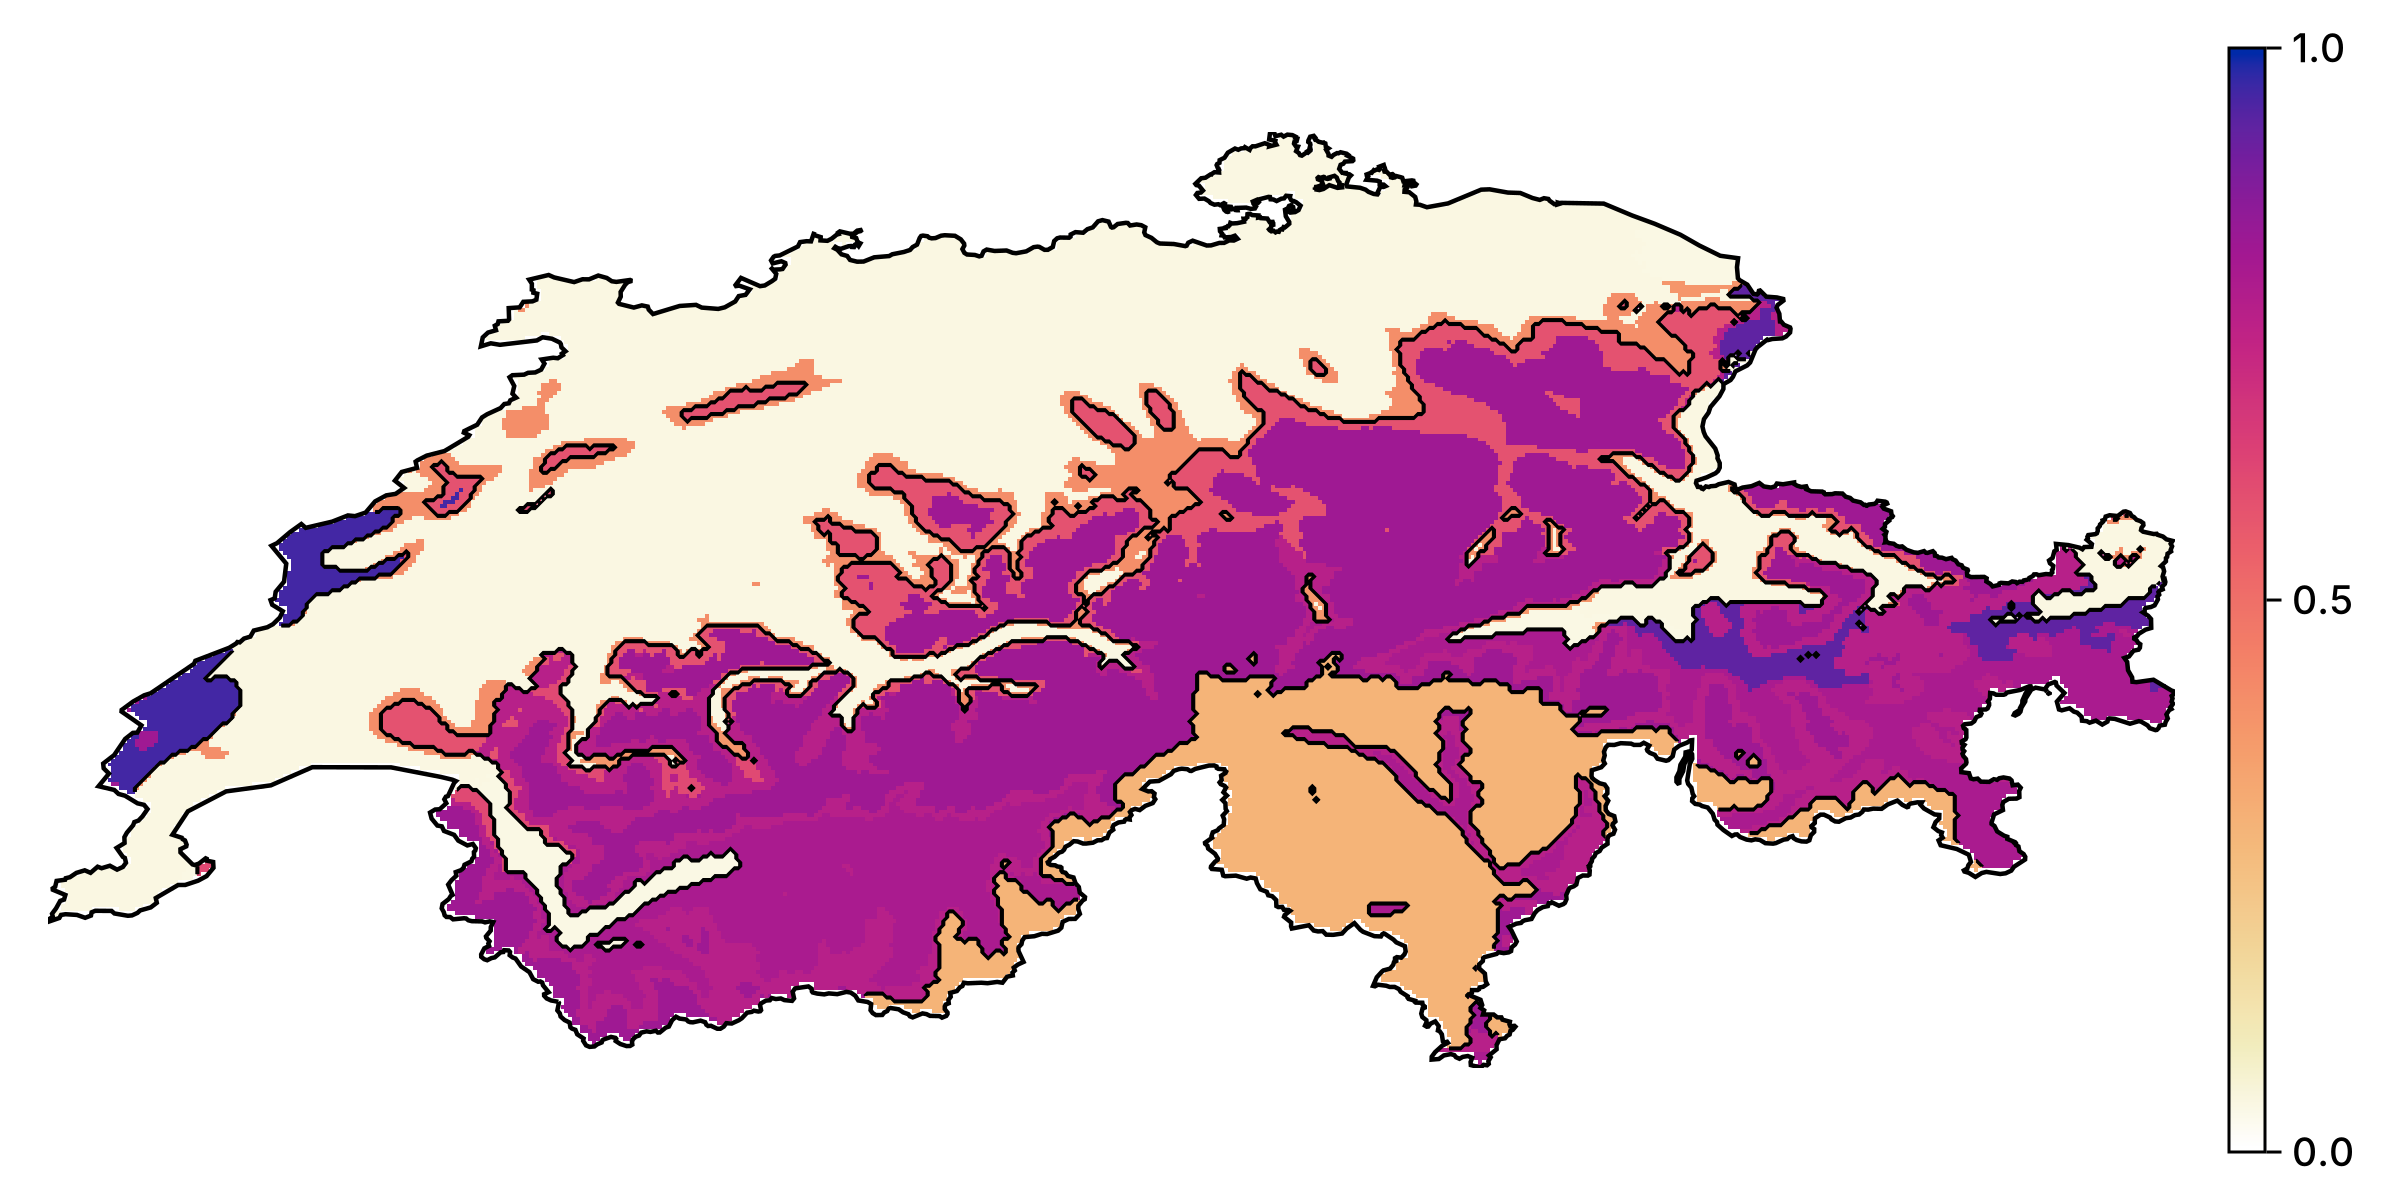
\includegraphics[keepaspectratio]{figures/slides_12_1.png}}~
\end{frame}

\begin{frame}{Can we improve on this model?}
\phantomsection\label{can-we-improve-on-this-model}
variable selection

data transformation

hyper-parameters tuning

will focus on the later (same process for the two above)
\end{frame}

\begin{frame}{Moving theshold classification}
\phantomsection\label{moving-theshold-classification}
p plus \textgreater{} p minus means threshold is 0.5

is it?

how do we check this
\end{frame}

\begin{frame}{Learning curve for the threshold}
\phantomsection\label{learning-curve-for-the-threshold}
\pandocbounded{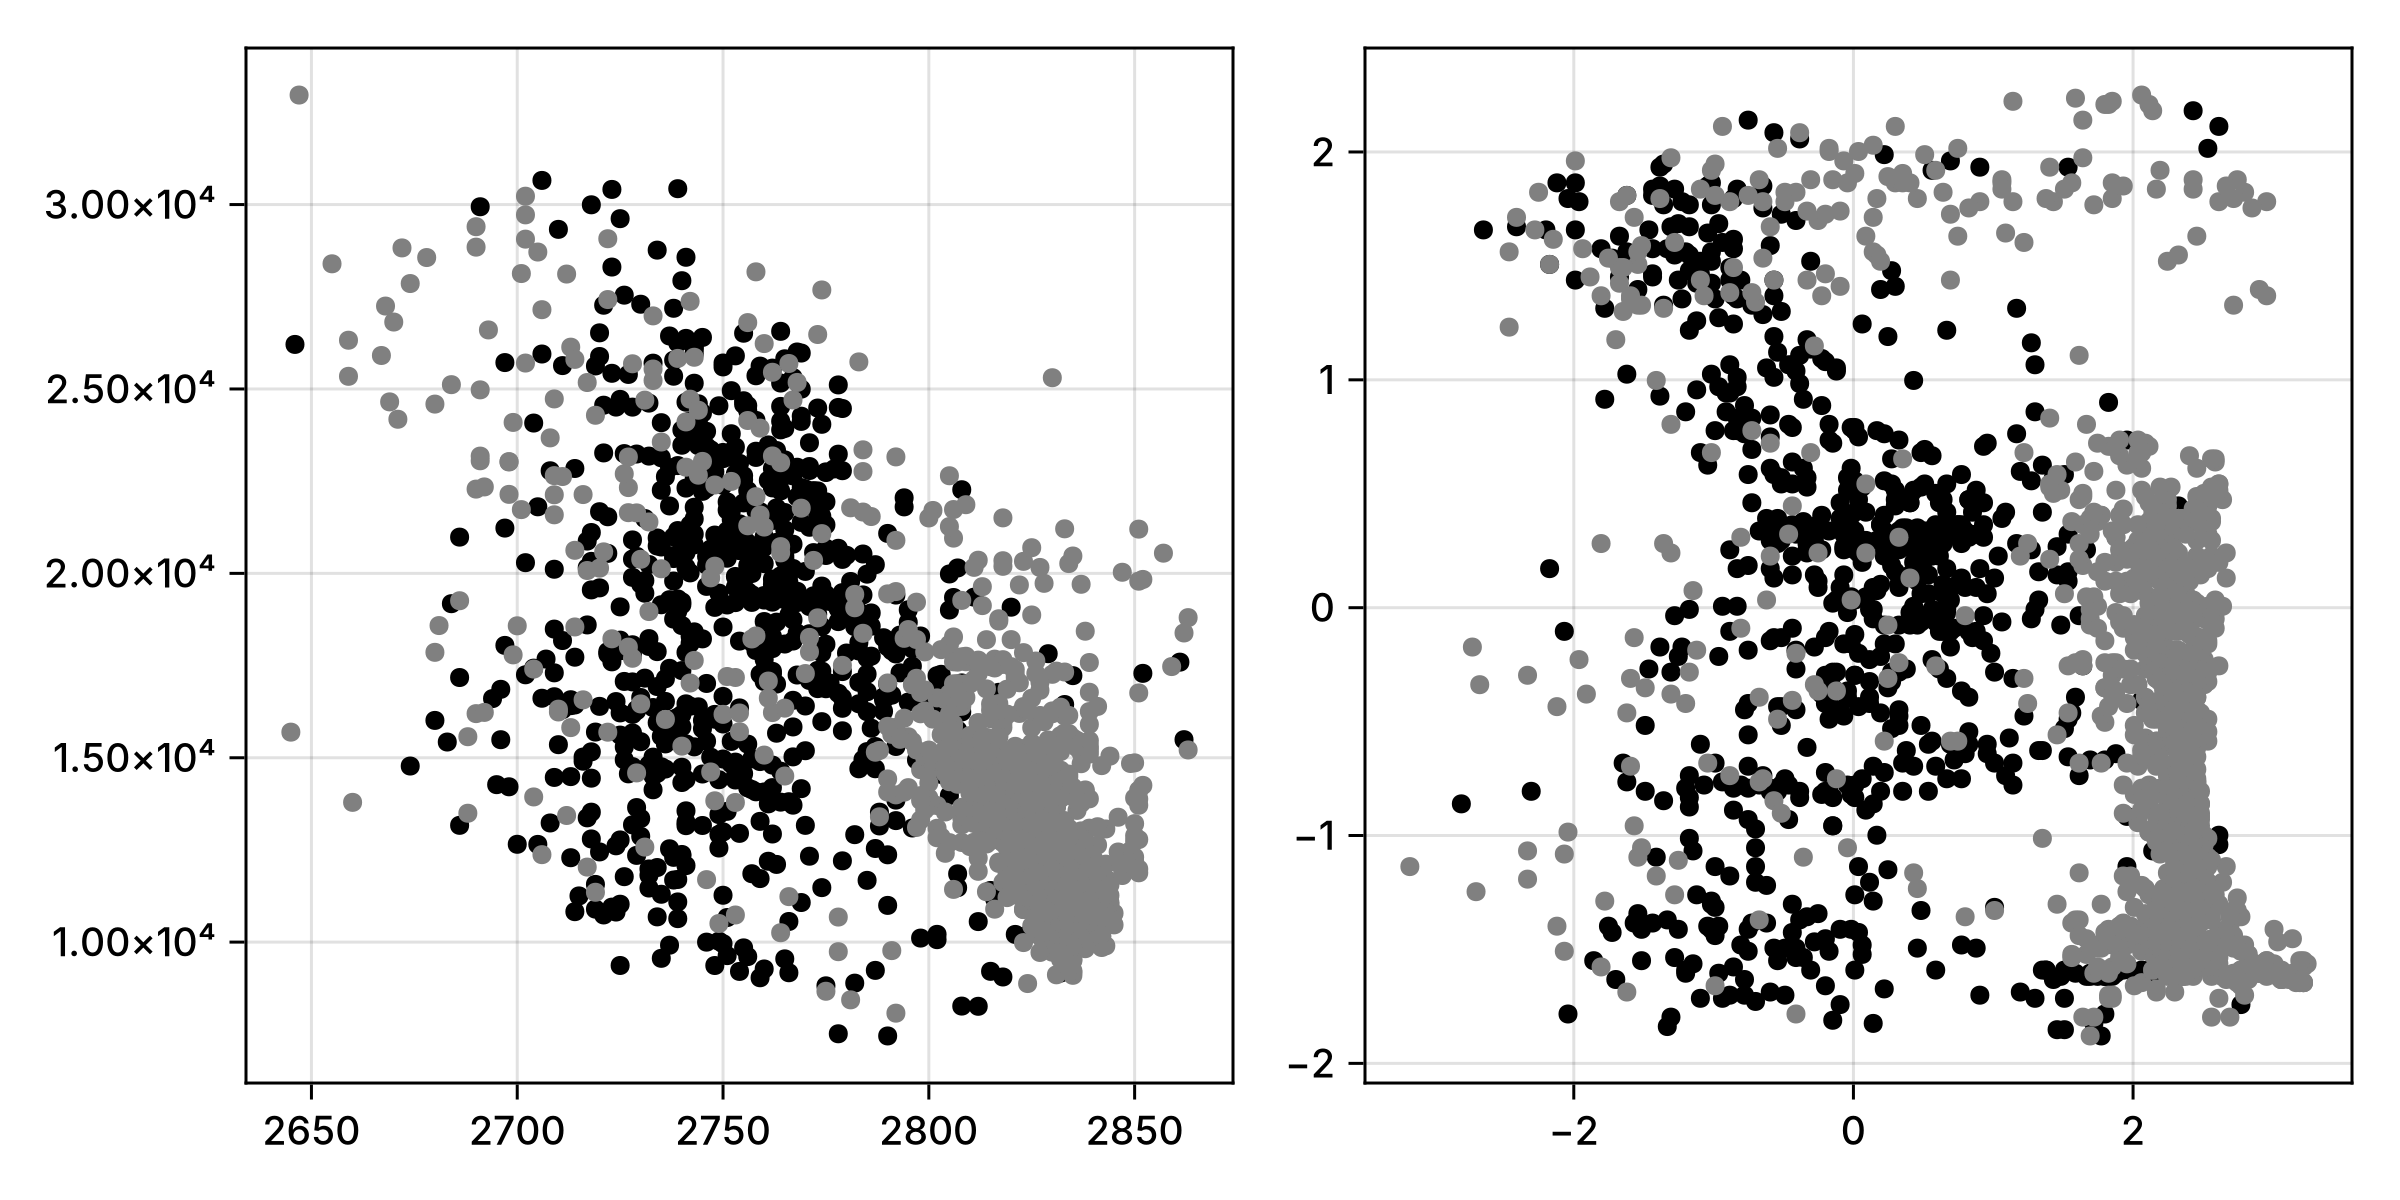
\includegraphics[keepaspectratio]{figures/slides_15_1.png}}~
\end{frame}

\begin{frame}{Receiver Operating Characteristic}
\phantomsection\label{receiver-operating-characteristic}
\pandocbounded{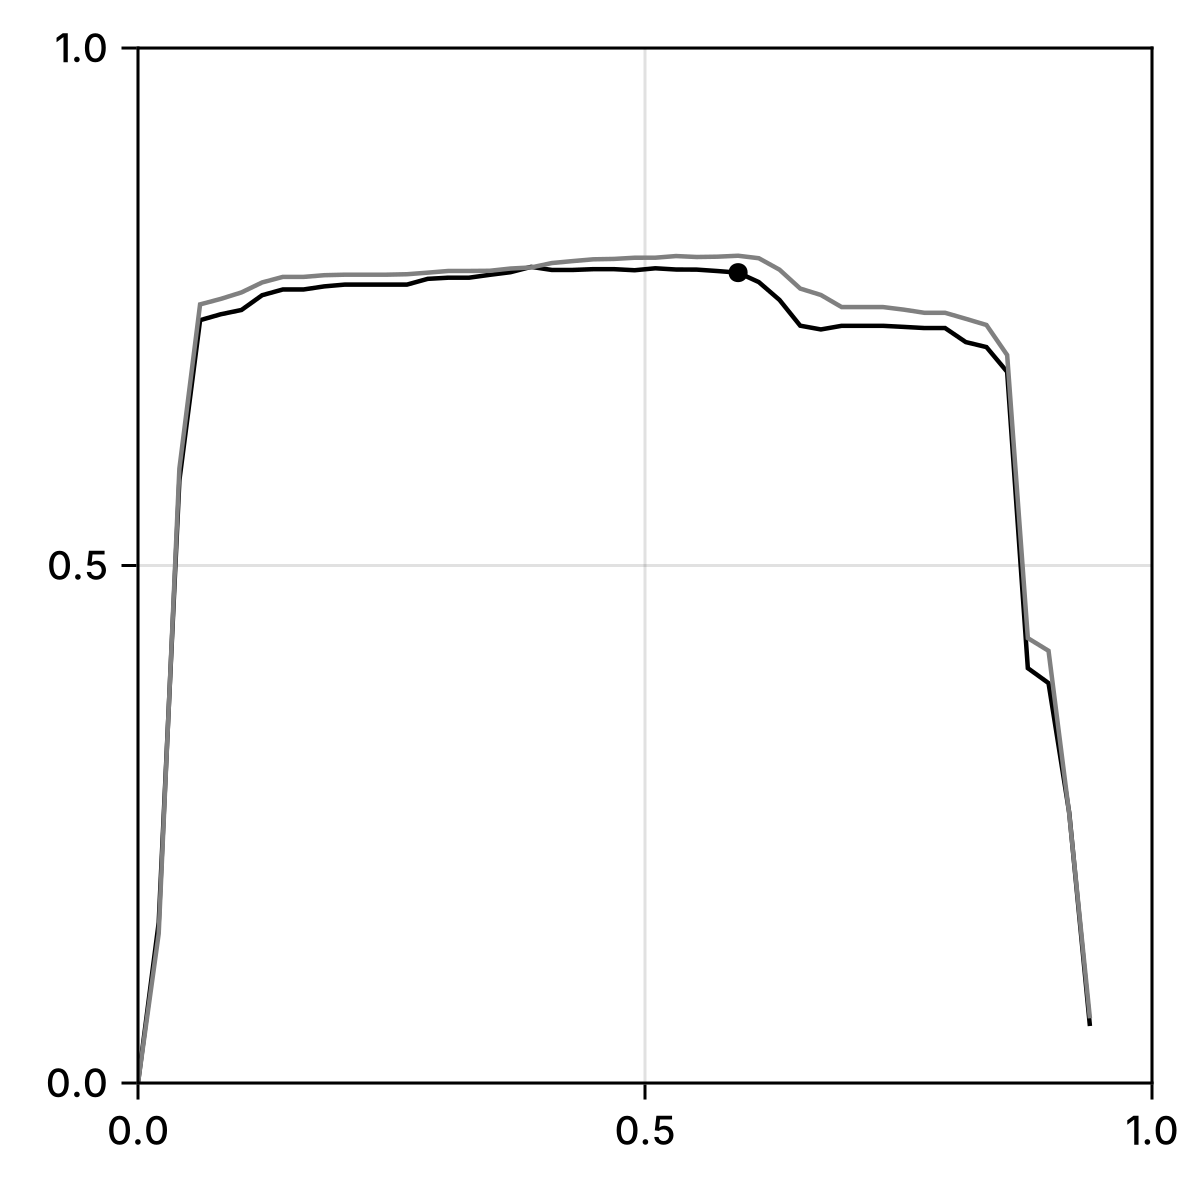
\includegraphics[keepaspectratio]{figures/slides_16_1.png}}~
\end{frame}

\begin{frame}{Precision-Recall Curve}
\phantomsection\label{precision-recall-curve}
\pandocbounded{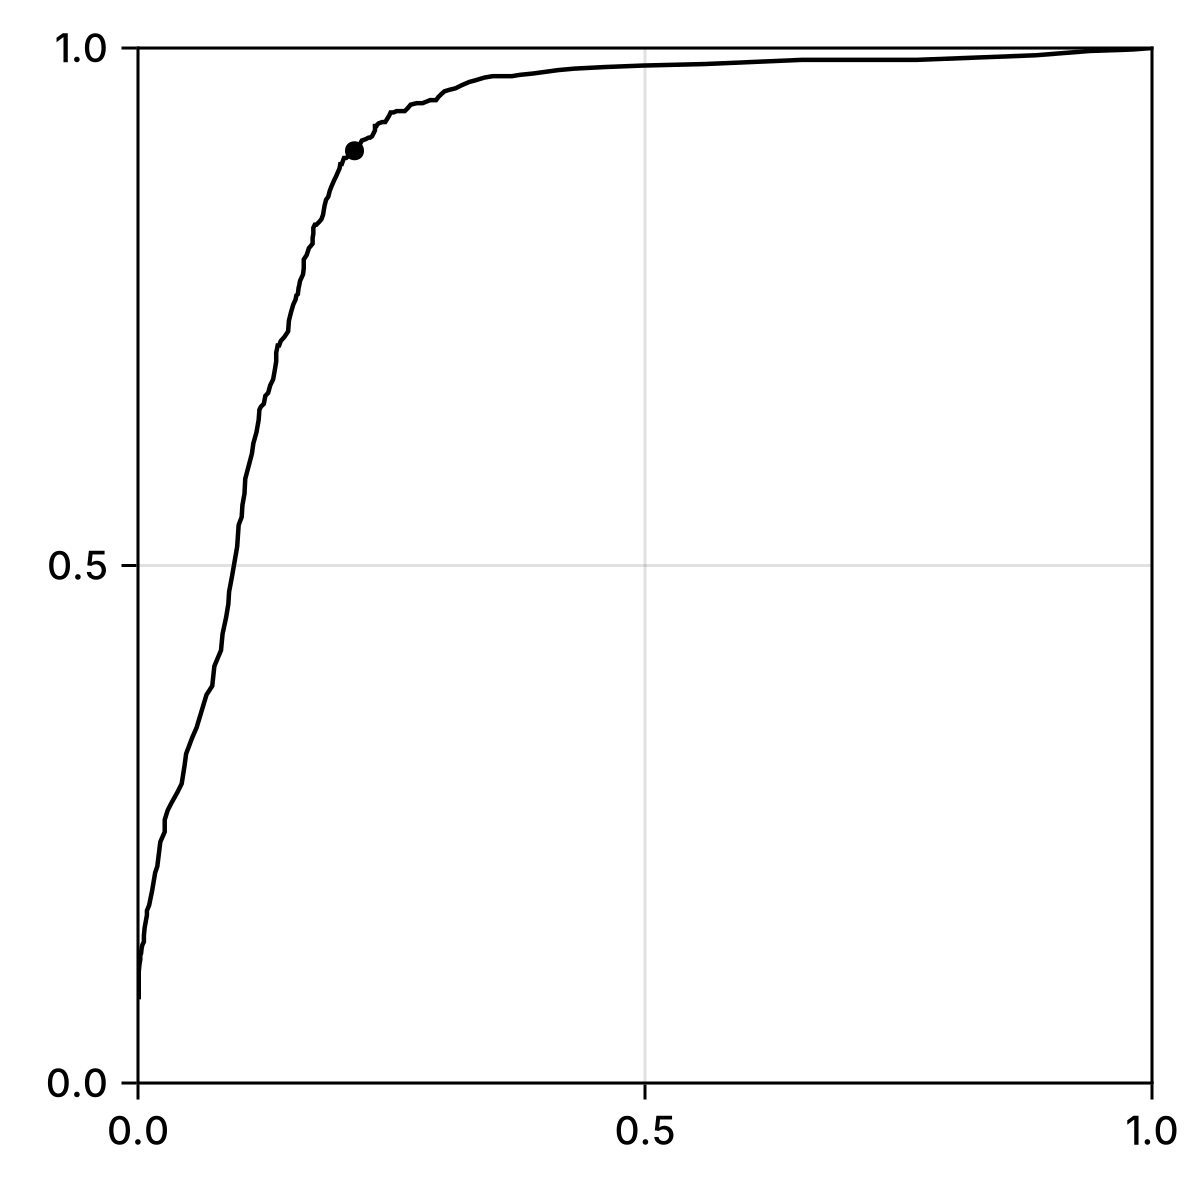
\includegraphics[keepaspectratio]{figures/slides_17_1.png}}~
\end{frame}

\begin{frame}{Revisting the model performance}
\phantomsection\label{revisting-the-model-performance}
\end{frame}

\begin{frame}{Updated prediction}
\phantomsection\label{updated-prediction}
\pandocbounded{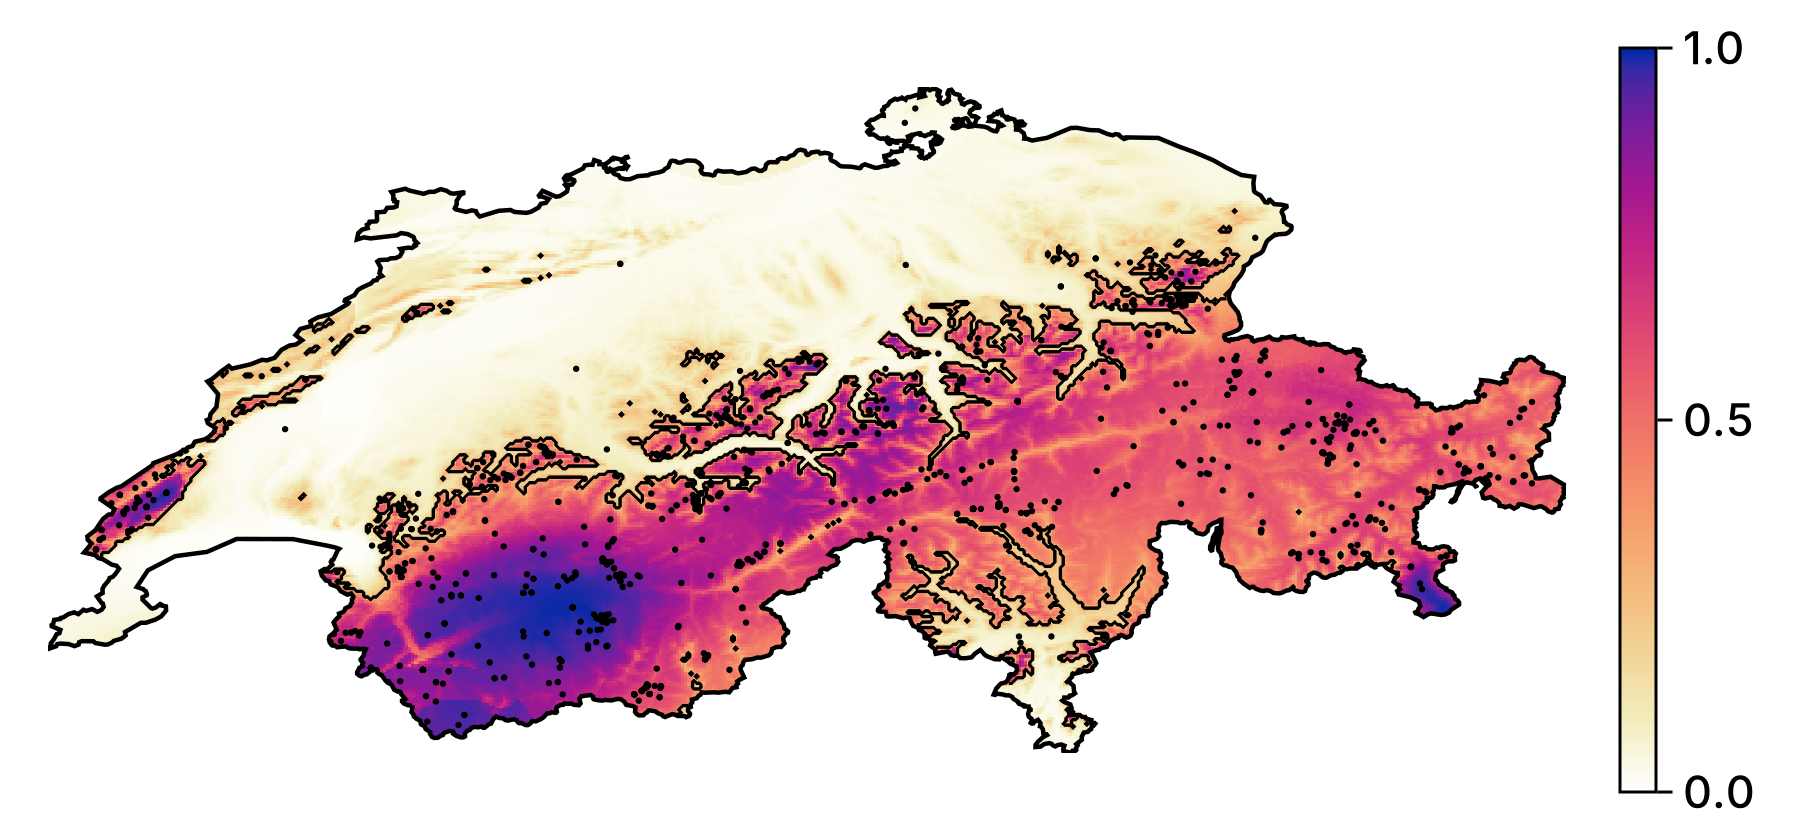
\includegraphics[keepaspectratio]{figures/slides_20_1.png}}~
\end{frame}

\begin{frame}{Variable importance}
\phantomsection\label{variable-importance}
\end{frame}

\section{But why?}\label{but-why-1}

\begin{frame}{Intro explainable}
\phantomsection\label{intro-explainable}
\end{frame}

\begin{frame}{An ecology tool: partial response curves}
\phantomsection\label{an-ecology-tool-partial-response-curves}
\end{frame}

\begin{frame}{Example with temperature}
\phantomsection\label{example-with-temperature}
\pandocbounded{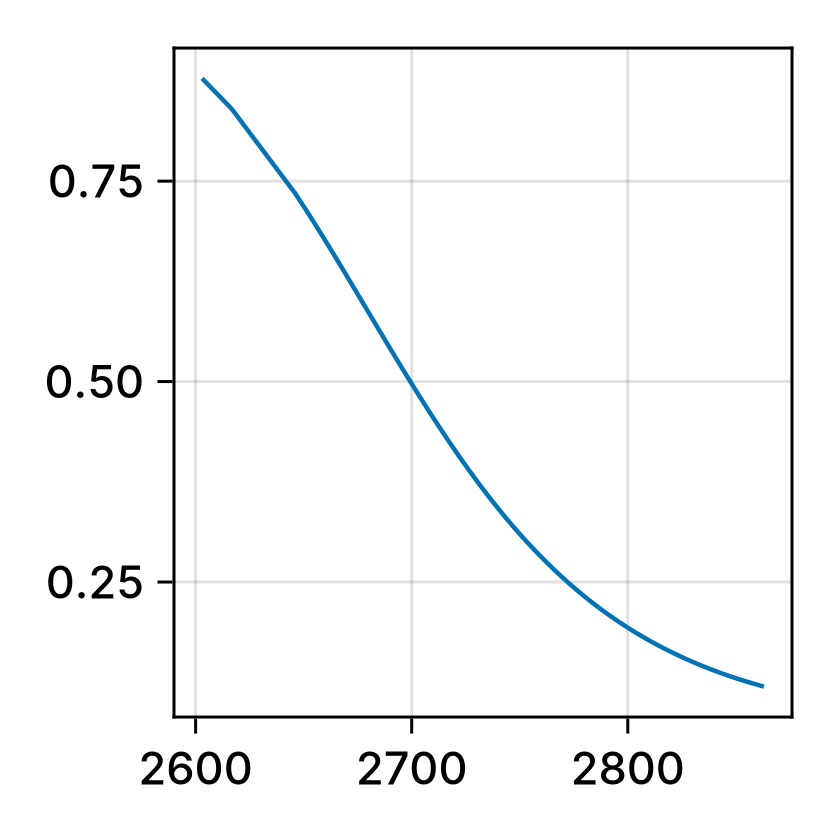
\includegraphics[keepaspectratio]{figures/slides_22_1.png}}~
\end{frame}

\begin{frame}{Example with two variables}
\phantomsection\label{example-with-two-variables}
\pandocbounded{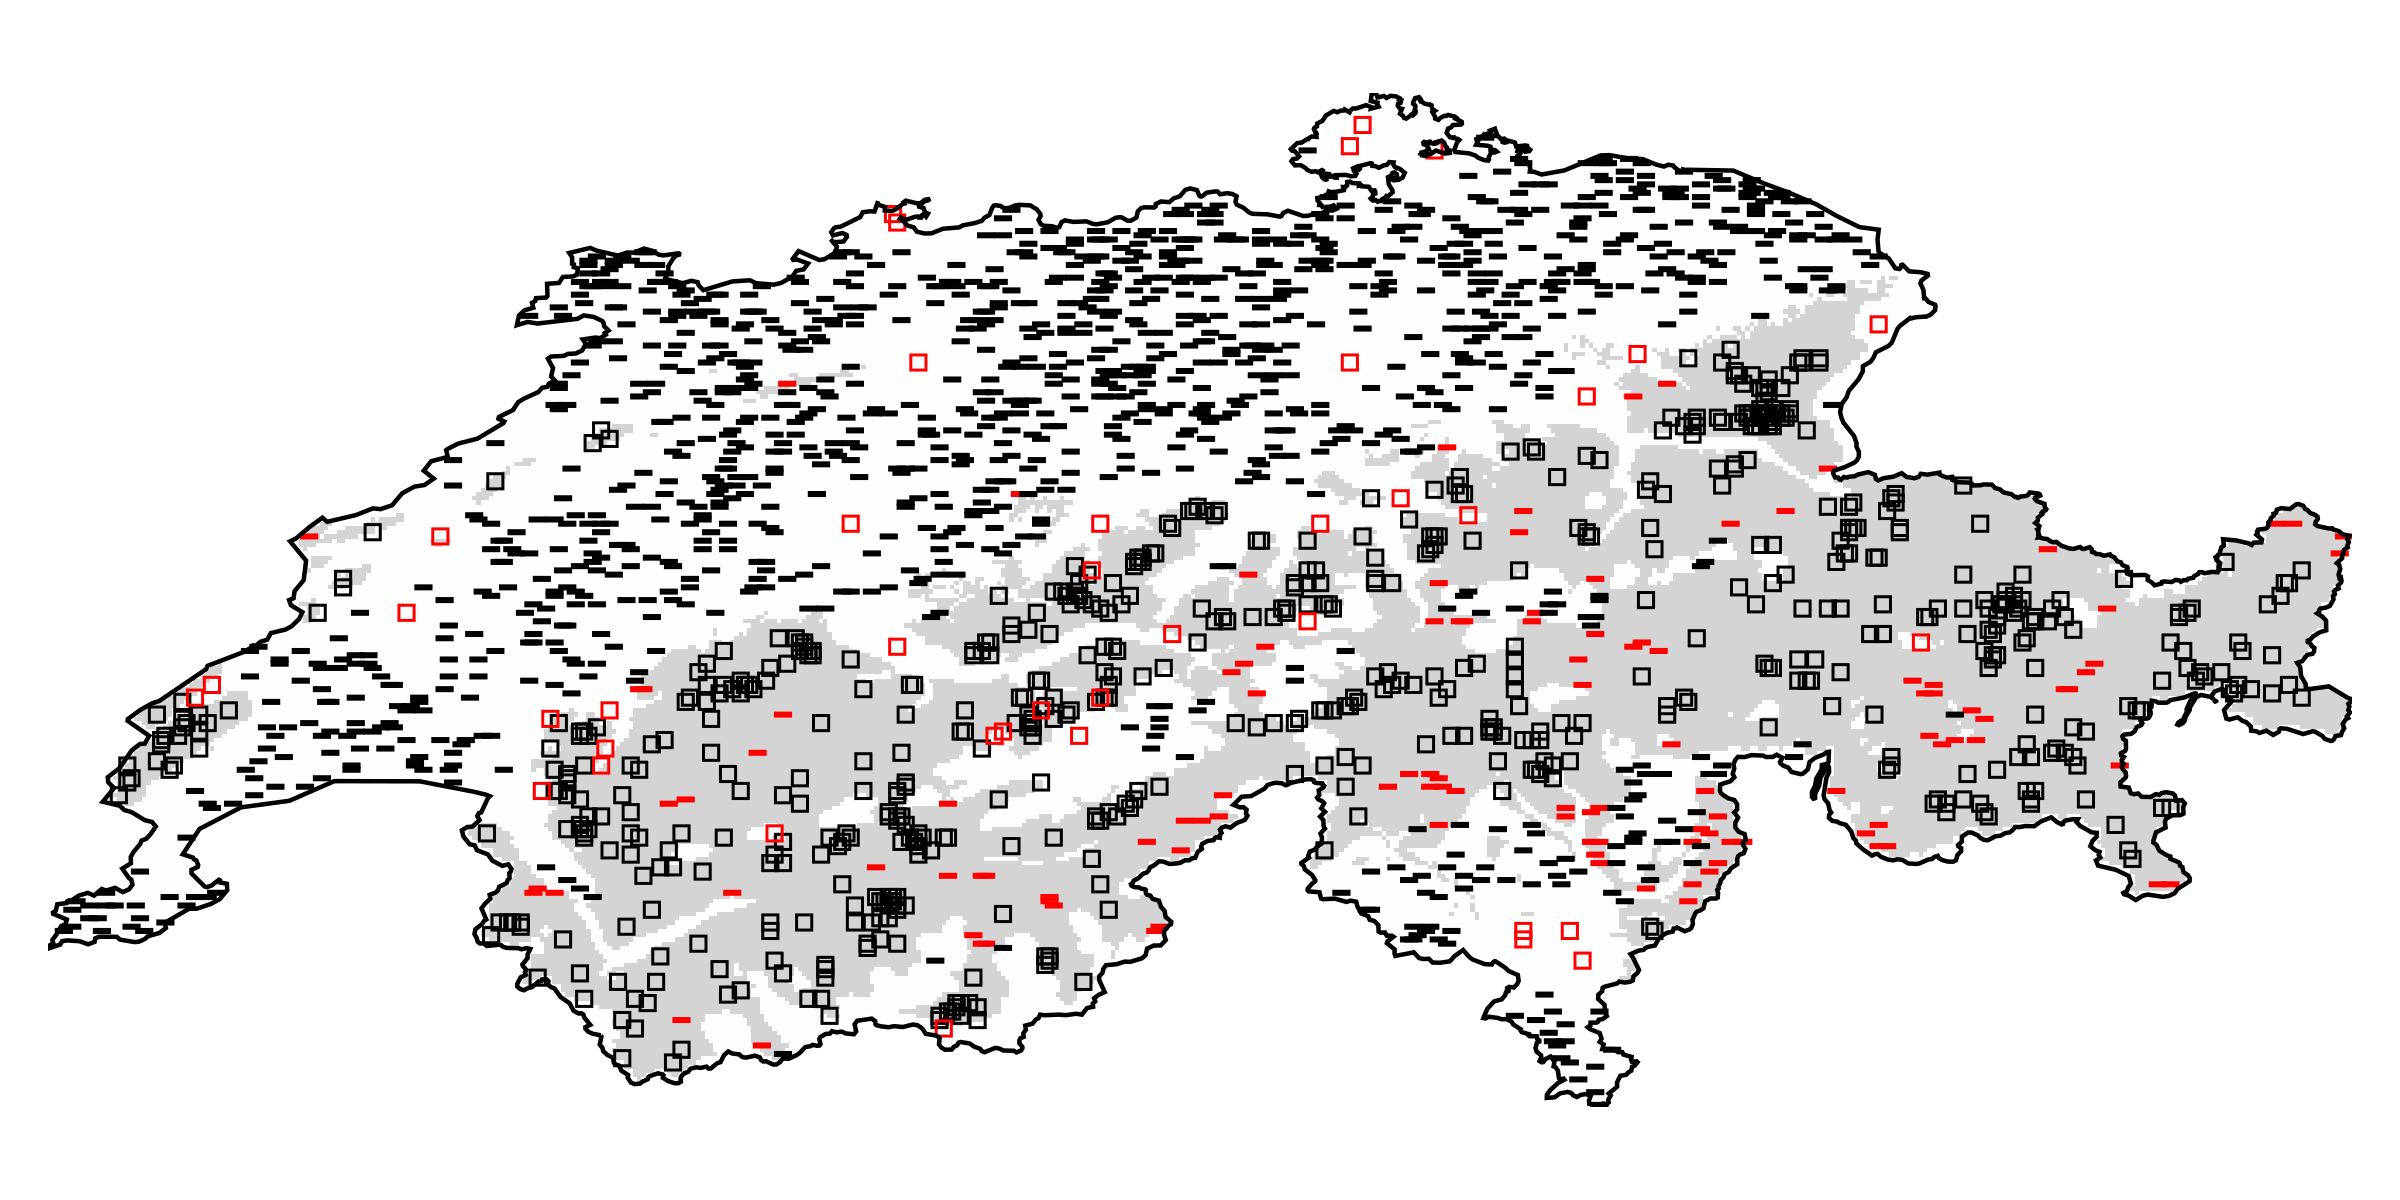
\includegraphics[keepaspectratio]{figures/slides_23_1.png}}~
\end{frame}

\begin{frame}{Spatialized partial response plot}
\phantomsection\label{spatialized-partial-response-plot}
\pandocbounded{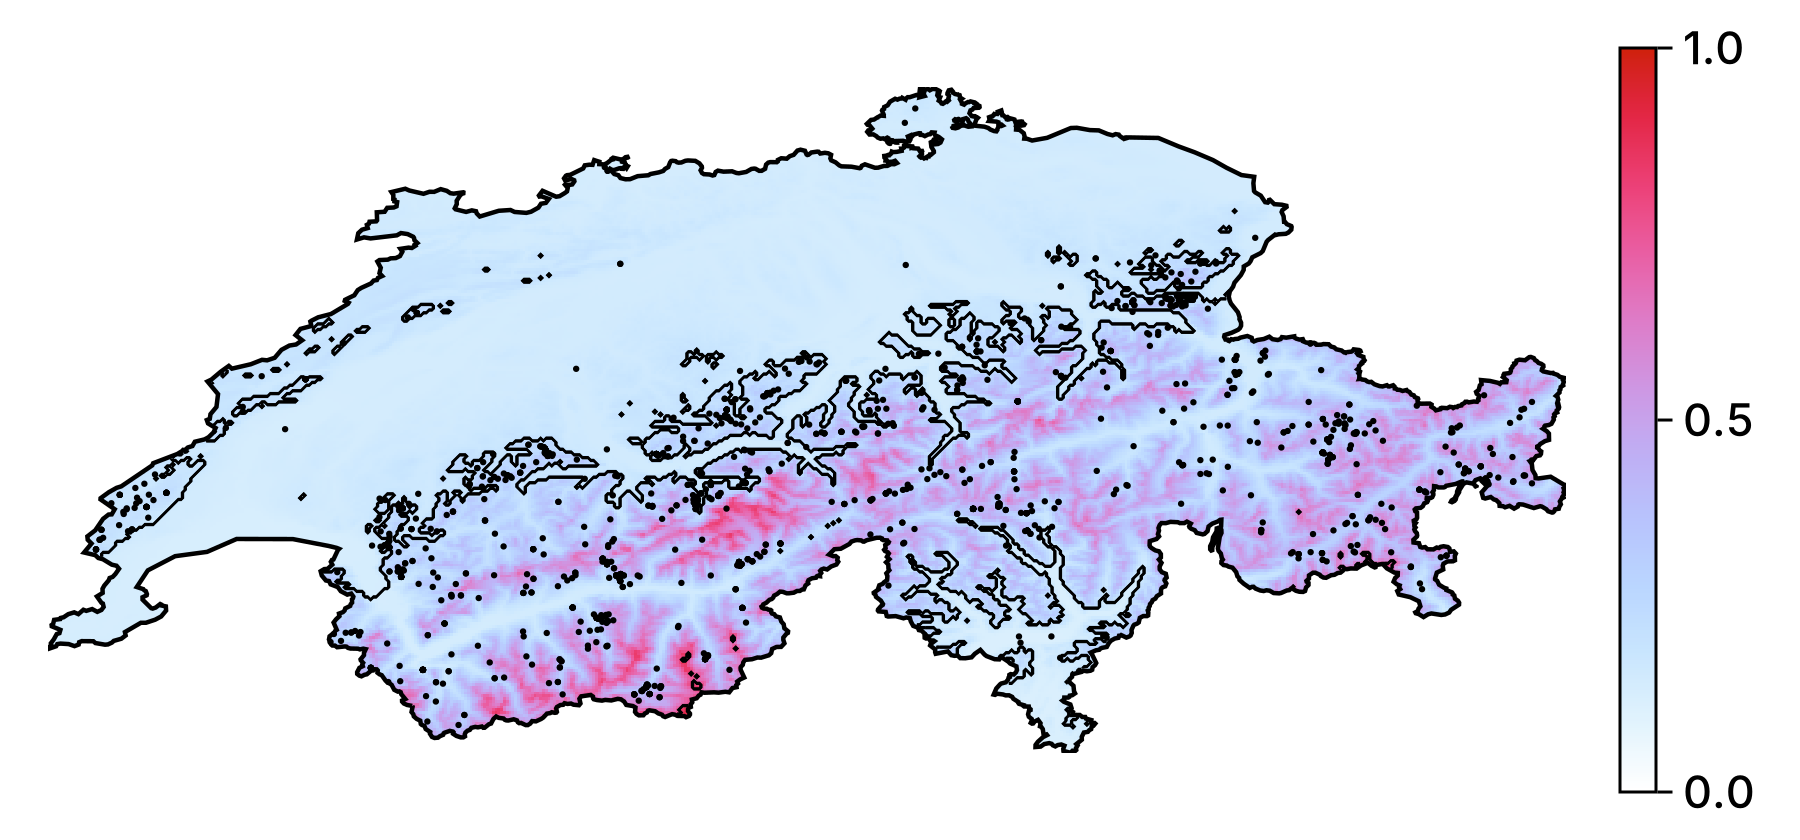
\includegraphics[keepaspectratio]{figures/slides_24_1.png}}~
\end{frame}

\begin{frame}{Spatialized partial response (binary outcome)}
\phantomsection\label{spatialized-partial-response-binary-outcome}
\pandocbounded{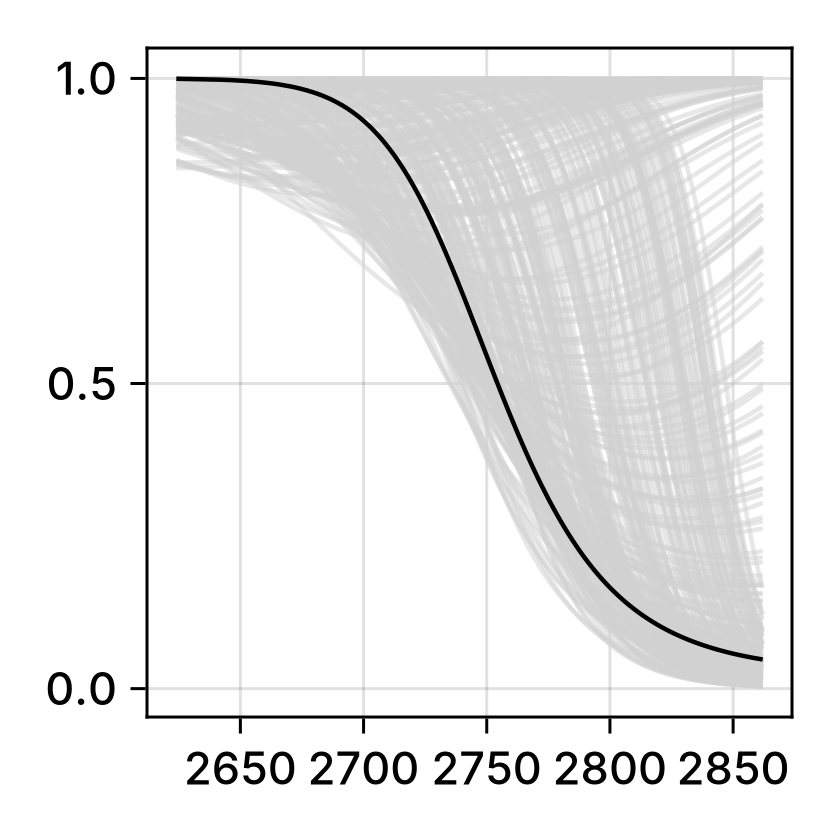
\includegraphics[keepaspectratio]{figures/slides_25_1.png}}~
\end{frame}

\begin{frame}{Inflated response curves}
\phantomsection\label{inflated-response-curves}
Averaging the variables is \alert{masking a lot of variability}!

Alternative solution:

\begin{enumerate}
\tightlist
\item
  Generate a grid for all the variables
\item
  For all combinations in this grid, use it as the stand-in for the
  variables to replace
\end{enumerate}

In practice: Monte-Carlo on a reasonable number of samples.
\end{frame}

\begin{frame}{Example}
\phantomsection\label{example}
\pandocbounded{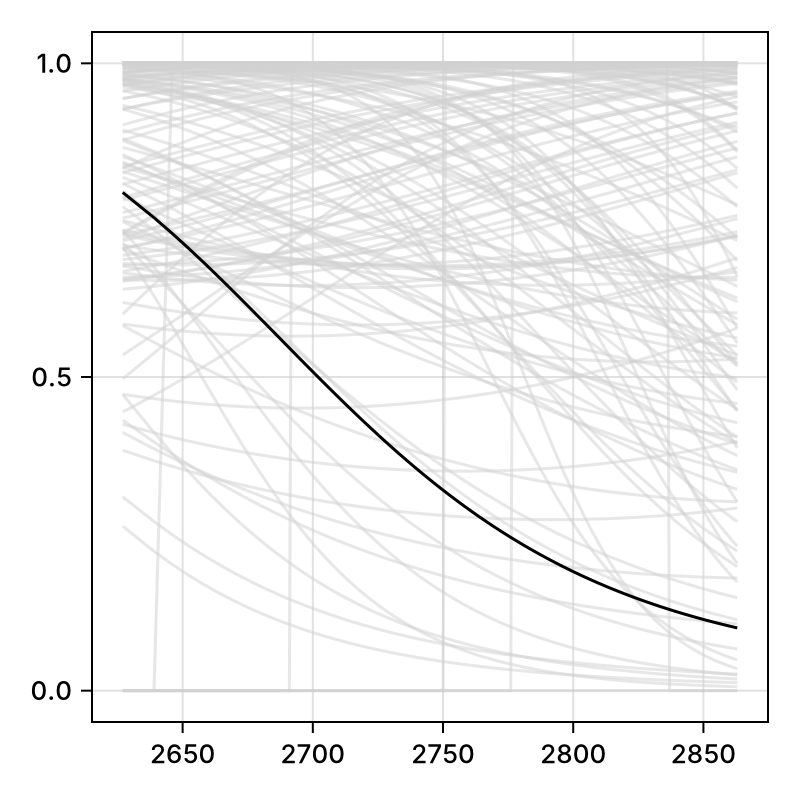
\includegraphics[keepaspectratio]{figures/slides_26_1.png}}~
\end{frame}

\begin{frame}{Limitations}
\phantomsection\label{limitations}
\begin{itemize}
\tightlist
\item
  partial responses can only generate model-level information
\item
  they break the structure of values for all predictors at the scale of
  a single observation
\item
  their interpretation is unclear
\end{itemize}
\end{frame}

\begin{frame}{Shapley}
\phantomsection\label{shapley}
\end{frame}

\begin{frame}{Example}
\phantomsection\label{example-1}
\end{frame}

\begin{frame}{Response curves revisited}
\phantomsection\label{response-curves-revisited}
\pandocbounded{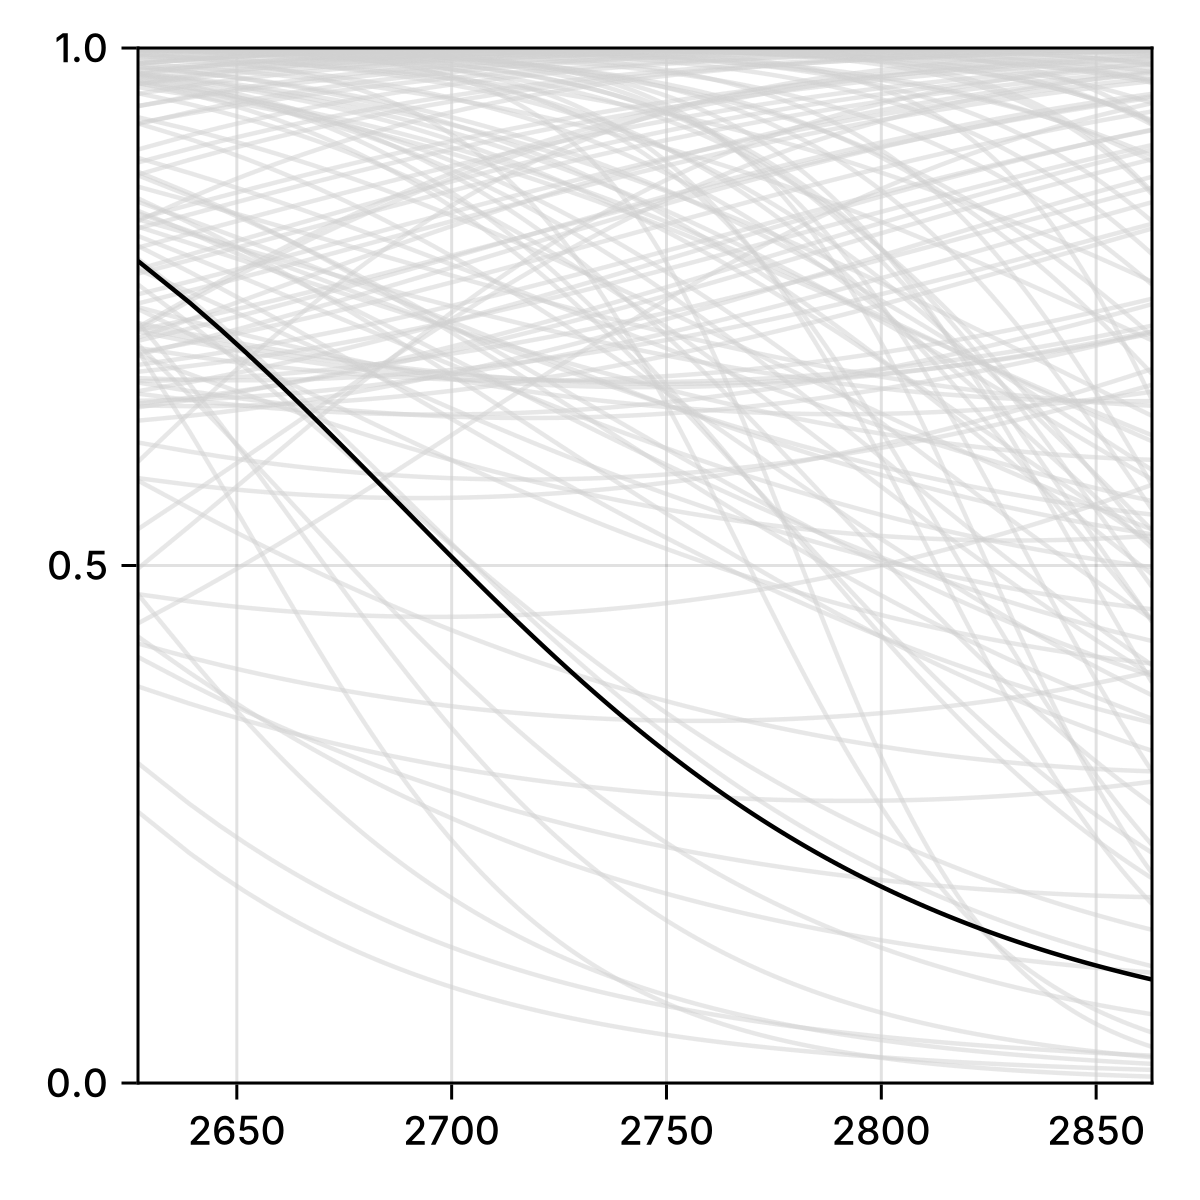
\includegraphics[keepaspectratio]{figures/slides_28_1.png}}~
\end{frame}

\begin{frame}{On a map}
\phantomsection\label{on-a-map}
\pandocbounded{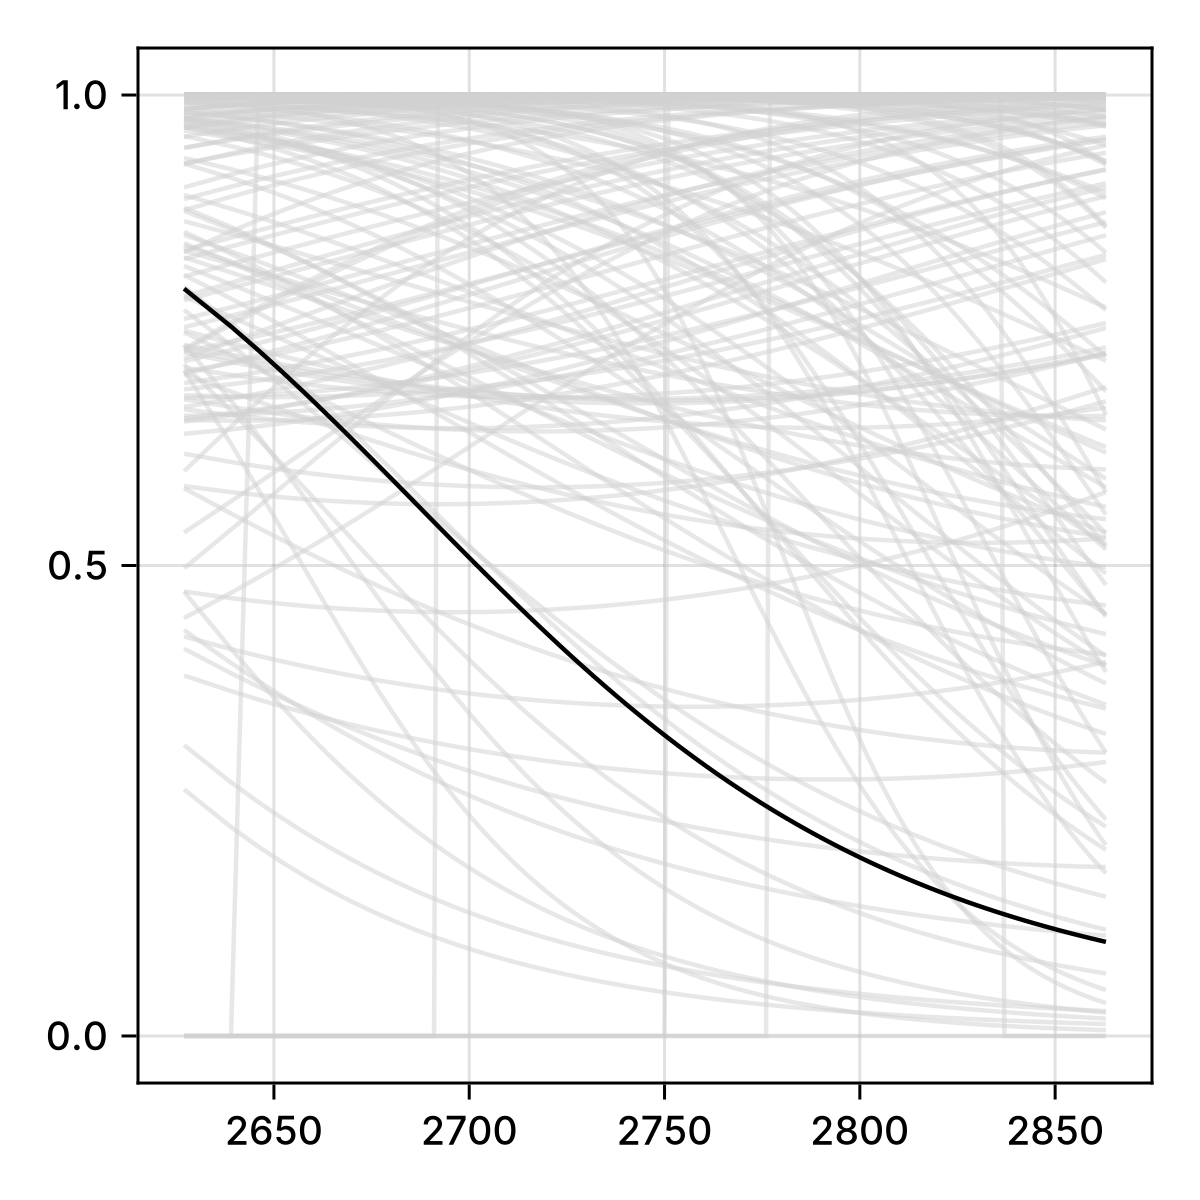
\includegraphics[keepaspectratio]{figures/slides_29_1.png}}~
\end{frame}

\begin{frame}{Variable importance revisited}
\phantomsection\label{variable-importance-revisited}
with shapley
\end{frame}

\begin{frame}{Most important predictor}
\phantomsection\label{most-important-predictor}
mosaic map
\end{frame}

\section{What if?}\label{what-if}

\begin{frame}{Intro to counterfactuals}
\phantomsection\label{intro-to-counterfactuals}
what they are
\end{frame}

\section{Ensemble models}\label{ensemble-models}

\section{Conclusions}\label{conclusions}

\end{document}
